\documentclass[border=10pt]{standalone}
\usepackage{tikz}\usepackage{amsmath}\usetikzlibrary{arrows.meta}
\begin{document}
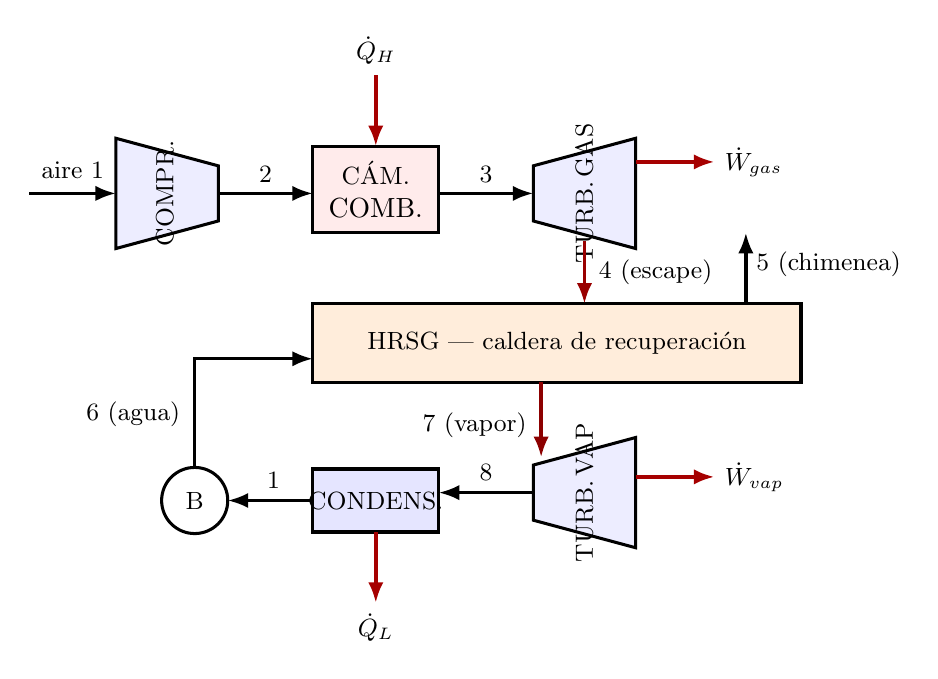
\begin{tikzpicture}[line width=1pt,>={Latex[length=2.6mm]}]
  % ===================== CICLO DE GAS (arriba) =====================
  % compresor
  \fill[blue!7] (0,3.8)--(0,5.2)--(1.3,4.85)--(1.3,4.15)--cycle;
  \draw[line width=1.1pt] (0,3.8)--(0,5.2)--(1.3,4.85)--(1.3,4.15)--cycle;
  \node[rotate=90] at (0.62,4.5){\small COMPR.};
  % camara de combustion
  \fill[red!8] (2.5,4.0) rectangle (4.1,5.1); \draw[line width=1.1pt] (2.5,4.0) rectangle (4.1,5.1);
  \node[align=center] at (3.3,4.55){\small CÁM.\\COMB.};
  % turbina de gas
  \fill[blue!7] (5.3,4.15)--(5.3,4.85)--(6.6,5.2)--(6.6,3.8)--cycle;
  \draw[line width=1.1pt] (5.3,4.15)--(5.3,4.85)--(6.6,5.2)--(6.6,3.8)--cycle;
  \node[rotate=90] at (5.95,4.5){\small TURB.\,GAS};
  % ===================== HRSG (banda central) =====================
  \fill[orange!14] (2.5,2.1) rectangle (8.7,3.1); \draw[line width=1.1pt] (2.5,2.1) rectangle (8.7,3.1);
  \node at (5.6,2.6){\small HRSG --- caldera de recuperación};
  % ===================== CICLO DE VAPOR (abajo) =====================
  % turbina de vapor
  \fill[blue!7] (5.3,0.35)--(5.3,1.05)--(6.6,1.4)--(6.6,0.0)--cycle;
  \draw[line width=1.1pt] (5.3,0.35)--(5.3,1.05)--(6.6,1.4)--(6.6,0.0)--cycle;
  \node[rotate=90] at (5.95,0.7){\small TURB.\,VAP};
  % condensador
  \fill[blue!10] (2.5,0.2) rectangle (4.1,1.0); \draw[line width=1.1pt] (2.5,0.2) rectangle (4.1,1.0);
  \node at (3.3,0.6){\small CONDENS.};
  % bomba
  \draw[line width=1.1pt] (1.0,0.6) circle (0.42); \node at (1.0,0.6){\small B};
  % ---------- tuberias del gas ----------
  \draw[->,line width=1.2pt] (-1.1,4.5)--(0,4.5); \node[above] at (-0.55,4.55){\small aire 1};
  \draw[->,line width=1.2pt] (1.3,4.5)--(2.5,4.5); \node[above] at (1.9,4.5){\small 2};
  \draw[->,line width=1.2pt] (4.1,4.5)--(5.3,4.5); \node[above] at (4.7,4.5){\small 3};
  \draw[->,red!65!black,line width=1.3pt] (3.3,6.0)--(3.3,5.1); \node[above] at (3.3,6.0){\small $\dot Q_H$};
  \draw[->,red!65!black,line width=1.3pt] (6.6,4.9)--(7.6,4.9); \node[right] at (7.6,4.9){\small $\dot W_{gas}$};
  \draw[->,red!60!black,line width=1.2pt] (5.95,3.9)--(5.95,3.1); \node[right] at (6.0,3.5){\small 4 (escape)};
  \draw[->,line width=1.2pt] (8.0,3.1)--(8.0,4.0); \node[right] at (8.0,3.6){\small 5 (chimenea)};
  % ---------- tuberias del vapor ----------
  \draw[->,red!55!black,line width=1.2pt] (5.4,2.1)--(5.4,1.15); \node[left] at (5.35,1.55){\small 7 (vapor)};
  \draw[->,red!65!black,line width=1.3pt] (6.6,0.9)--(7.6,0.9); \node[right] at (7.6,0.9){\small $\dot W_{vap}$};
  \draw[->,line width=1.2pt] (5.3,0.7)--(4.1,0.7); \node[above] at (4.7,0.72){\small 8};
  \draw[->,red!65!black,line width=1.3pt] (3.3,0.2)--(3.3,-0.7); \node[below] at (3.3,-0.7){\small $\dot Q_L$};
  \draw[->,line width=1.2pt] (2.5,0.6)--(1.42,0.6); \node[above] at (2.0,0.62){\small 1};
  \draw[->,line width=1.2pt] (1.0,1.02)--(1.0,2.4)--(2.5,2.4); \node[left] at (0.95,1.7){\small 6 (agua)};
\end{tikzpicture}
\end{document}
